\documentclass{beamer}
\usepackage{ctex} % 支持中文
\usepackage{graphicx} % 加载图形处理宏包
\usepackage{booktabs} % 用于美化表格线条
\usepackage{listings} % 代码高亮
\usepackage[dvipsnames]{xcolor} % 更多彩色支持
\usepackage{tikz} % 绘图支持
\usepackage{tabularx} % 支持表格宽度设置

% 设置代码高亮样式
\lstset{
    basicstyle=\ttfamily\small, % 设置字体族和大小
    breaklines=true, % 自动换行
    keywordstyle=\bfseries\color{NavyBlue}, % 设置关键字为粗体,颜色为 NavyBlue
    commentstyle=\itshape\color{black!50!white}, % 设置注释样式,斜体,浅灰色
    stringstyle=\bfseries\color{PineGreen!90!black}, % 设置字符串样式
    columns=flexible,
    frame=single, % 边框
    framesep=1em, % 设置代码与边框的距离
    tabsize=4
}

% 主题设置
\usetheme{Warsaw}
\title{ztest: A Unit Test Framework with GUI}
\author{郑辰阳}
\date{\today}

\begin{document}

\begin{frame}
    \titlepage
\end{frame}

\begin{frame}{需求分析}
    \begin{itemize}
        \item 随着复杂系统架构设计能力的培养需求日益凸显,掌握面向对象设计原则与模式化工程实践已成为高级软件工程教育的核心目标。
        \item 我们团队计划开发一个提供一个灵活、高效且易于使用(带图形用户界面GUI)的测试工具,旨在提供一个直观、易用的环境,方便开发人员和测试人员编写、运行和管理测试用例。
    \end{itemize}
\end{frame}

\begin{frame}{系统功能}
    \begin{itemize}
        \item 提供一个灵活、高效且易于使用(带图形用户界面GUI)的测试工具。
        \item 支持测试用例的管理、断言验证、测试执行以及结果报告。
        \item 支持多种测试类型(如单元测试、集成测试等),并提供详细的测试结果报告。
    \end{itemize}
\end{frame}

\begin{frame}{测试用例管理}
    \begin{itemize}
        \item \textbf{测试用例的定义}:通过继承 \textbf{ZtestBase} 类或使用模板类 \textbf{ZtestSingleCase} 定义测试用例。
        \item \textbf{测试用例的注册}:使用测试注册中心 \textbf{ZTestRegistry} 动态注册测试用例。
        \item \textbf{测试套件的构建}:通过 \textbf{ZTestSuite} 类组织多个测试用例,支持批量运行。
    \end{itemize}
\end{frame}

\begin{frame}{断言机制}
    \begin{itemize}
        \item \textbf{EXPECT\_EQ}:验证两个值是否相等。
        \item \textbf{ASSERT\_TRUE}:验证条件是否为真。
        \item \textbf{异常处理}:如果断言失败,抛出 \textbf{ZTestFailureException} 异常。
    \end{itemize}
\end{frame}

\begin{frame}{测试执行器}
    \begin{itemize}
        \item \textbf{ZTestContext}:测试上下文管理类,负责维护测试用例队列,并通过多线程并行执行测试。
        \item \textbf{ZTimer}:用于计时测试的运行时间。
        \item \textbf{测试结果收集}:测试结果存储在 \textbf{ZTestResult} 类中。
    \end{itemize}
\end{frame}

\begin{frame}{结果报告}
    \begin{itemize}
        \item \textbf{ZTestResult}:封装单个测试的结果信息。
        \item \textbf{测试套件报告}:通过 \textbf{ZTestSuite} 类生成测试套件的汇总报告。
        \item \textbf{日志输出}:测试结果通过 \textbf{ZLogger} 类输出到控制台。
    \end{itemize}
\end{frame}

\begin{frame}{整体架构}
    \begin{itemize}
        \item 使用 MVC(Model-View-Controller)模式架构。
        \item View 关注用户所看见的 UI 并且提供交互。
        \item Controller 负责控制器作用于模型和视图上。
        \item Model 主要实现对于底层文件的建模。
    \end{itemize}
    \centering
    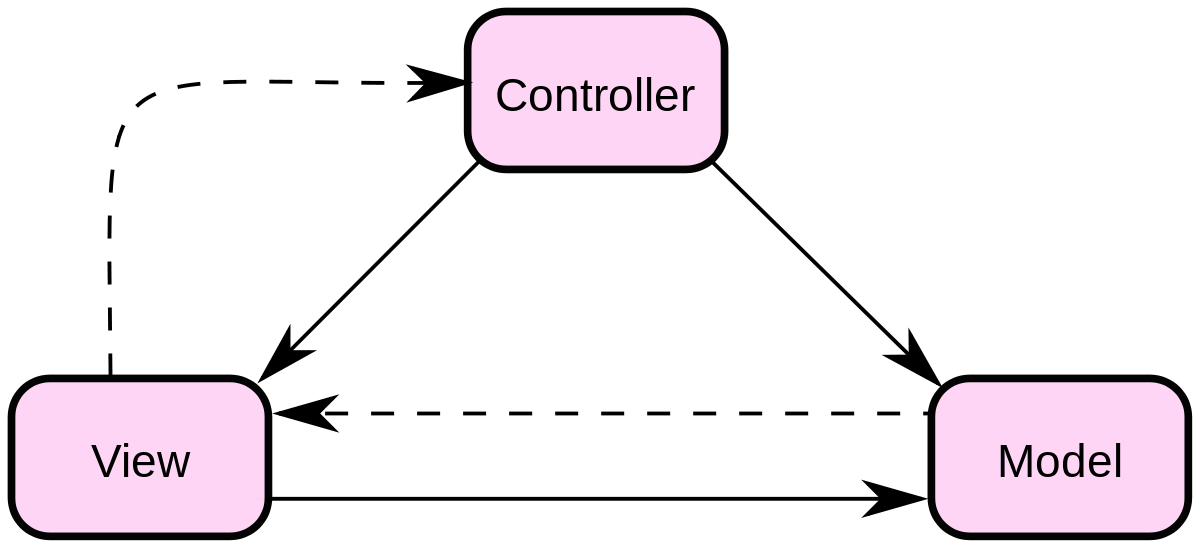
\includegraphics[width=0.6\textwidth]{img/mvc.png}
\end{frame}

\begin{frame}{技术细节}
    所有类都以Z开头。
    \begin{itemize}
        \item \textbf{ZtestInterface}:定义了测试用例的基本接口。
        \item \textbf{ZtestBase}:作为测试用例的基类,实现了测试的基本属性和方法。
        \item \textbf{ZtestSingleCase}:用于定义单个测试用例。
        \item \textbf{ZTestSuite}:用于组织多个测试用例。
        \item \textbf{ZTestRegistry}:测试注册中心,负责注册和管理测试用例。
        \item \textbf{ZTestContext}:测试上下文管理类。
    \end{itemize}
\end{frame}
\begin{frame}[fragile]{链式调用}
    工厂模式和构建器模式结合使用,实现链式调用。
    \begin{itemize}
        \item \textbf{TestFactory}:工厂类,帮助定义测试用例。
        \item \textbf{TestBuilder}:构建器类,用于构建测试用例。
    \end{itemize}
    \begin{lstlisting}[language=C++]
auto test_case = TestFactory::createTest("Addition", ZType::ZSAFE, "", add, 2, 3)
                    .setExpectedOutput(5)
                    .beforeAll([]() { logger.info("Initializing test case resources...\n"); })
                    .afterEach([]() { logger.info("Cleaning up after test...\n"); })
                    .build();
    \end{lstlisting}
\end{frame}
\begin{frame}[fragile]{类gtest的调用方式}
    使用宏展开,实现ASSERT\_TRUE和EXPECT\_EQ。
    \begin{lstlisting}[language=C++]
TEST(MathTests, Addition) {
    EXPECT_EQ(2 + 2, 4);
}
    \end{lstlisting}
\end{frame}

\begin{frame}{UI 实现}
    \begin{itemize}
        \item 使用 MVC 架构实现图形用户界面。
        \item 使用 Dear ImGui 框架构建可视化测试管理界面。
        \item 包括模型管理、视图渲染和控制器交互三部分。
    \end{itemize}
    \centering
    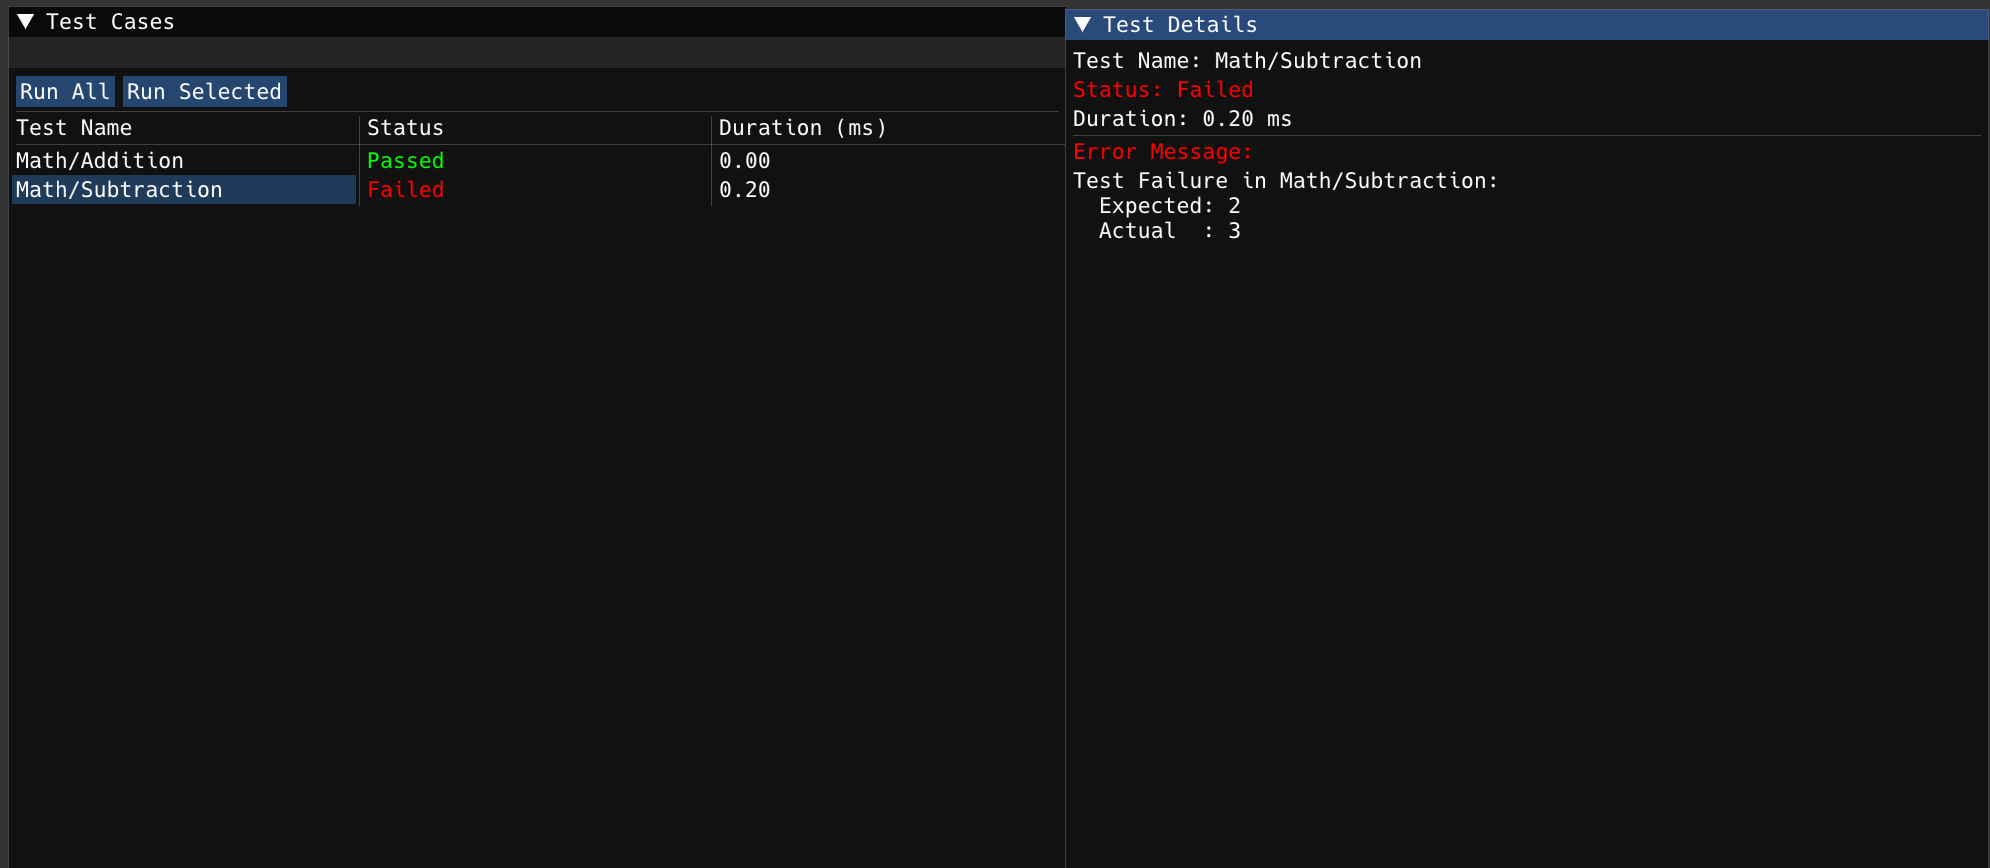
\includegraphics[width=0.8\textwidth]{img/ui.png}
\end{frame}
\begin{frame}{UML 类图}
    \begin{figure}[H]
        \centering
        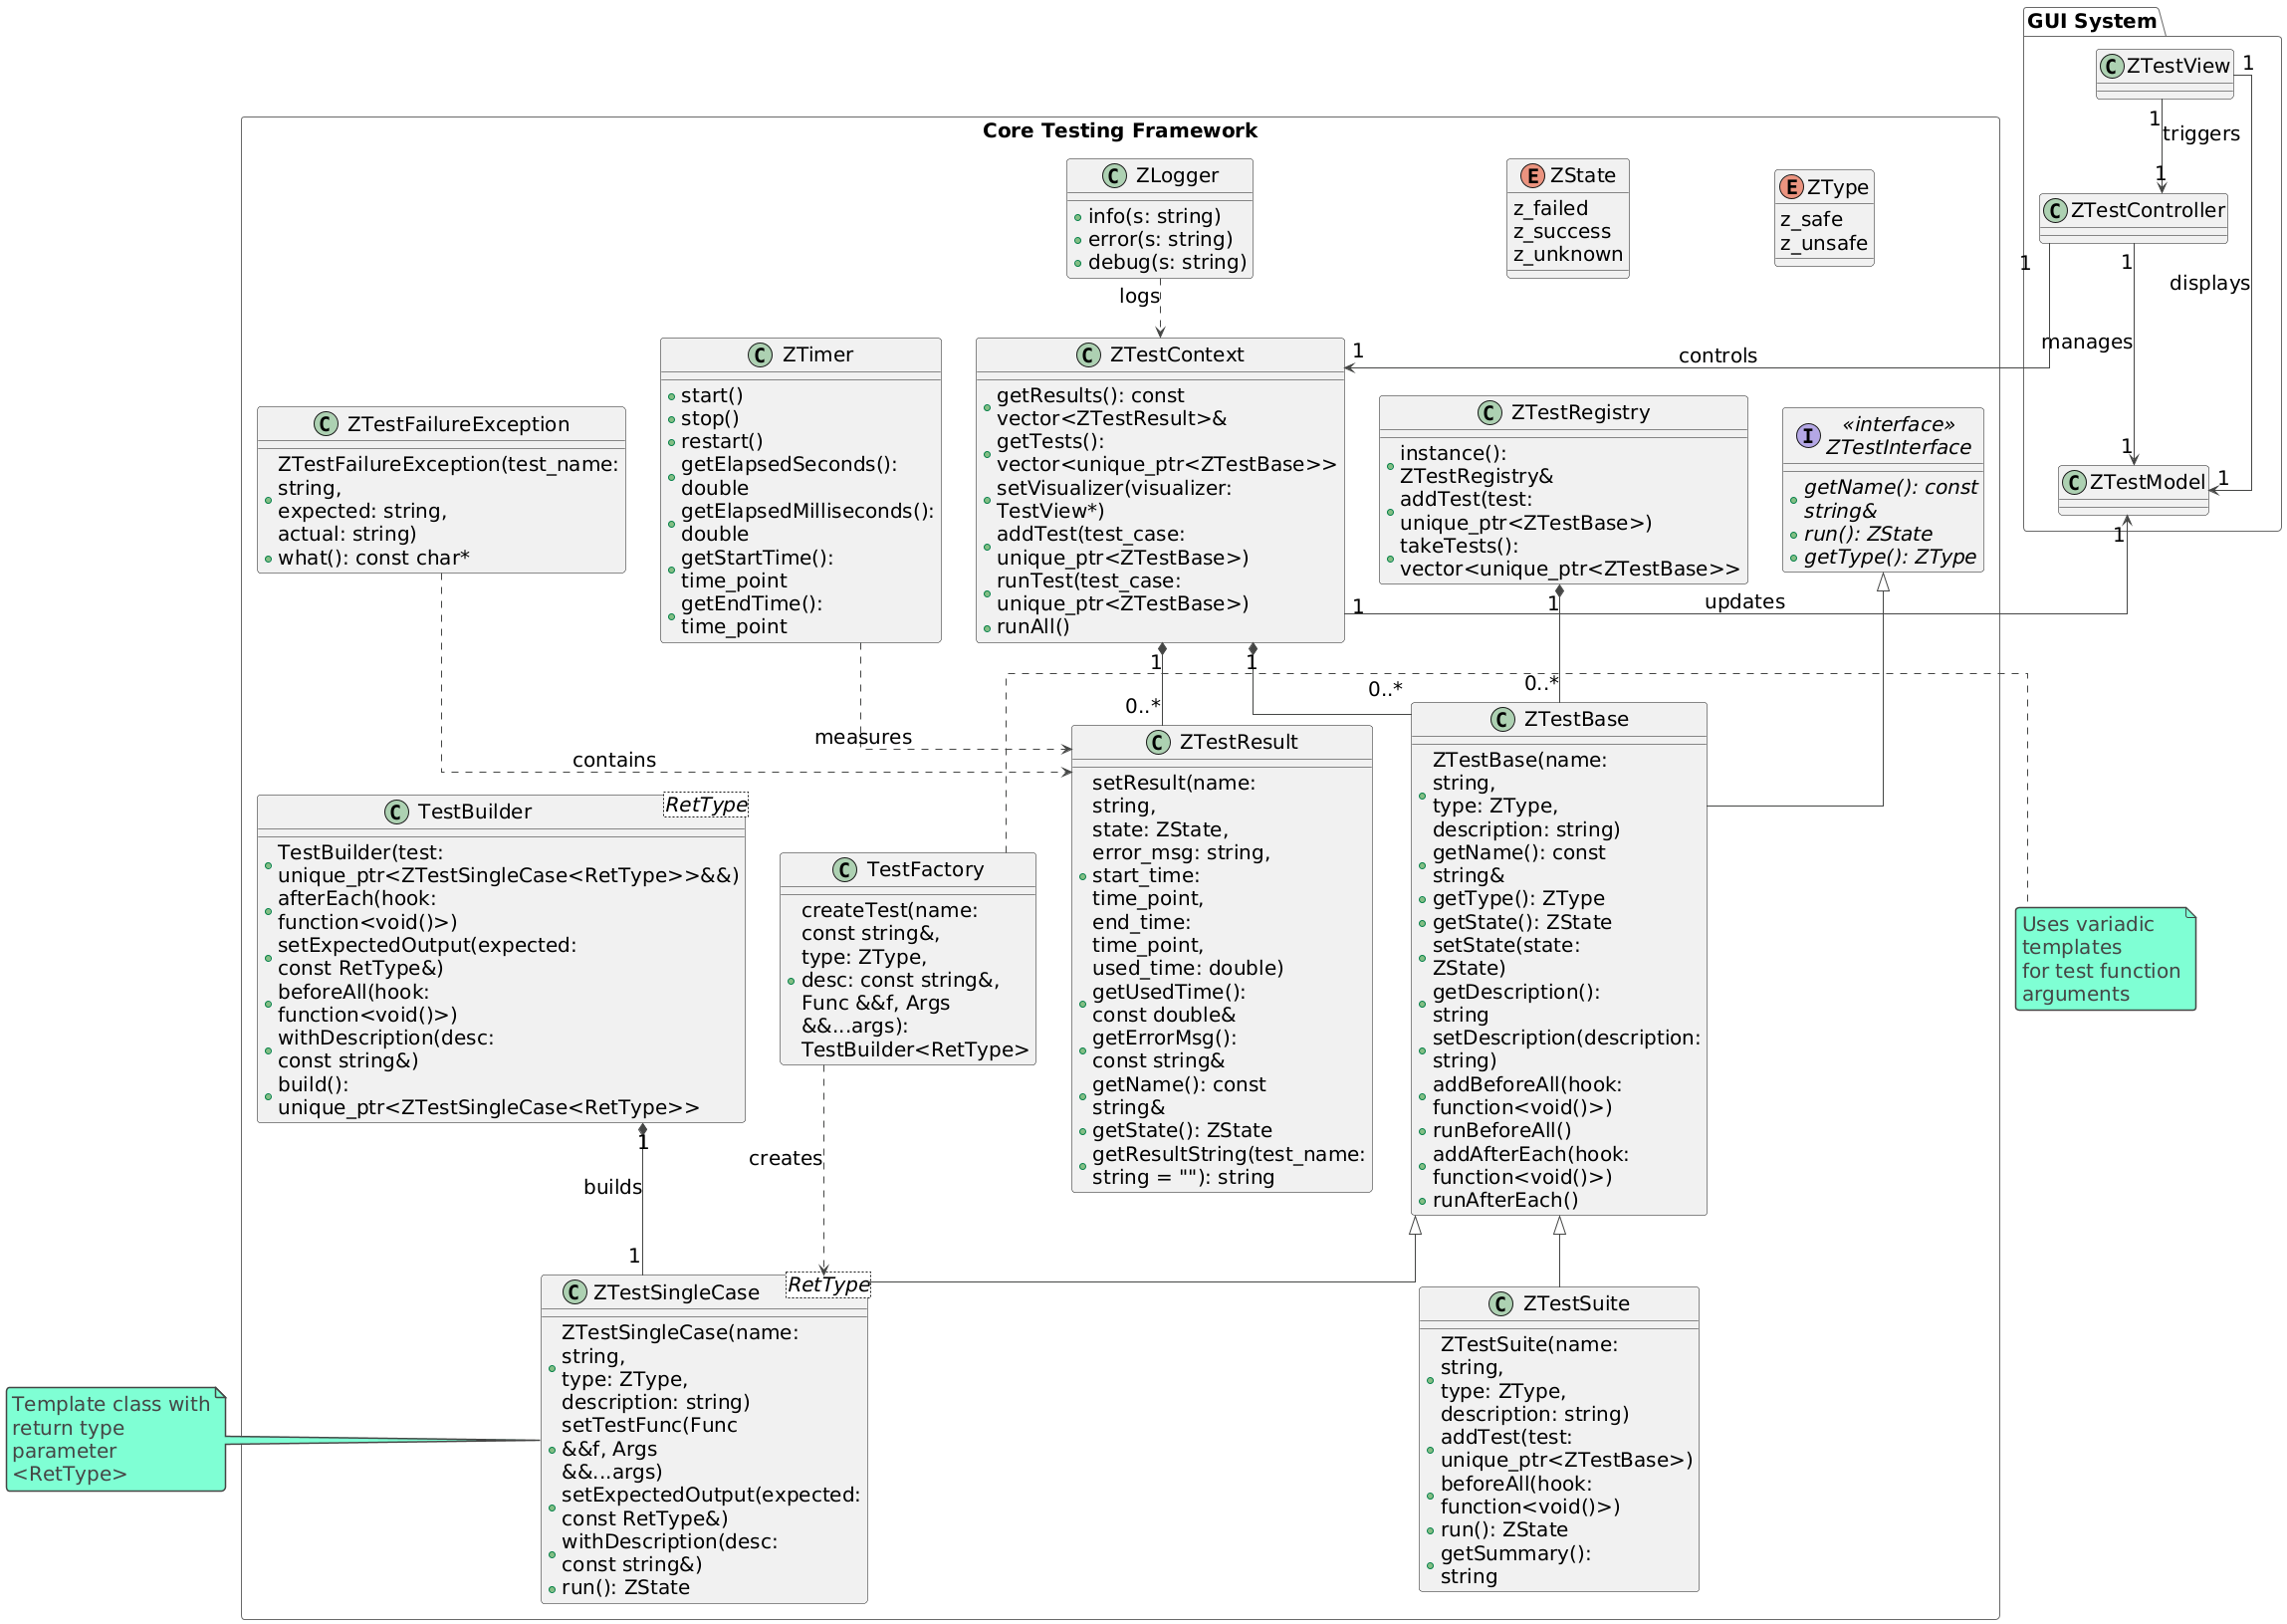
\includegraphics[width=\textwidth]{img/umlcore.png} % 插入图片
        \label{fig:diagram}
    \end{figure}
\end{frame}
\begin{frame}{MVC 类图}
    \begin{figure}[H]
        \centering
        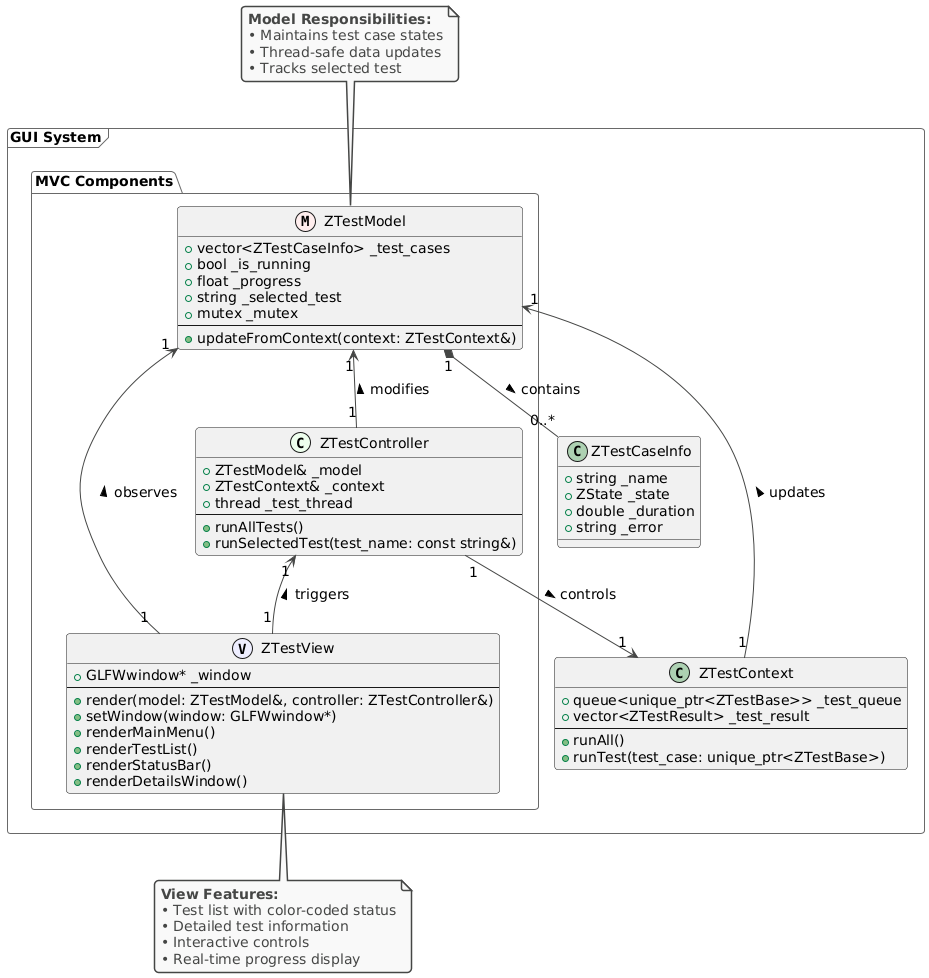
\includegraphics[width=0.7\textwidth]{img/umlgui.png} % 插入图片
        \label{fig:diagram}
    \end{figure}
\end{frame}
\begin{frame}{一些例子}
    \begin{itemize}
        \item 定义单个测试用例。
        \item 使用测试工厂创建测试用例。
        \item 构建测试套件。
        \item 运行测试并输出结果。
        \item 使用断言。
        \item 测试结果的输出。
        \item 动态注册测试用例。
    \end{itemize}
\end{frame}

\begin{frame}[fragile]{定义单个测试用例}
    \begin{lstlisting}[language=C++]
class MathTests_Addition : public ZtestBase {
public:
    MathTests_Addition()
        : ZtestBase("MathTests.Addition", ZType::ZSAFE, "Test addition function") {}

    Zstate run() override {
        EXPECT_EQ(5, add(2, 3)); // 预期结果为5
        EXPECT_EQ(0, add(0, 0)); // 预期结果为0
        return Zstate::Z_SUCCESS;
    }
};
    \end{lstlisting}
\end{frame}

\begin{frame}[fragile]{使用测试工厂创建测试用例}
    \begin{lstlisting}[language=C++]
auto test_case = TestFactory::createTest("Addition", ZType::ZSAFE, "", add, 2, 3)
                     .setExpectedOutput(5)
                     .beforeAll([]() { logger.info("Initializing test case resources...\n"); })
                     .afterEach([]() { logger.info("Cleaning up after test...\n"); })
                     .build();
    \end{lstlisting}
\end{frame}

\begin{frame}[fragile]{构建测试套件}
    \begin{lstlisting}[language=C++]
auto suite = std::make_unique<ZTestSuite>("MathTests", ZType::ZSAFE, "Mathematical operations tests");
suite->addTest(TestFactory::createTest("Addition", ZType::ZSAFE, "", add, 2, 3)
               .setExpectedOutput(5)
               .build());
suite->addTest(TestFactory::createTest("NegativeNumbers", ZType::ZSAFE, "", add, -2, -3)
               .setExpectedOutput(-5)
               .build());
    \end{lstlisting}
\end{frame}

\begin{frame}[fragile]{运行测试并输出结果}
    \begin{lstlisting}[language=C++]
ZTestContext context;
context.add_test(std::move(suite)); // 添加测试套件
context.run_all(); // 运行所有测试
    \end{lstlisting}
\end{frame}

\begin{frame}[fragile]{使用断言}
    \begin{lstlisting}[language=C++]
ZTEST_F(MathTests, Addition) {
    EXPECT_EQ(5, add(2, 3)); // 预期结果为5
    EXPECT_EQ(0, add(0, 0)); // 预期结果为0
    return Zstate::Z_SUCCESS;
}
    \end{lstlisting}
\end{frame}

\begin{frame}[fragile]{测试结果的输出}
    \begin{lstlisting}[language=C++]
ZTestResult result;
result.set_result(Zstate::Z_SUCCESS, "", start_time, end_time, elapsed_time);
logger.info(result.get_result_string("MathTests.Addition") + "\n");
    \end{lstlisting}
\end{frame}

\begin{frame}[fragile]{动态注册测试用例}
    \begin{lstlisting}[language=C++]
ZTEST_F(MathTests, NegativeNumbers) {
    ASSERT_TRUE(add(-2, -3) == -5); // 断言结果为-5
    return Zstate::Z_SUCCESS;
}
    \end{lstlisting}
\end{frame}

\end{document}